% Texto ou documento elaborado pelo autor, a fim de complementar sua argumentação, sem prejuízo da unidade nuclear do trabalho.

% ---
% Inicia os apêndices
% ---
\begin{apendicesenv}
	
	% Imprime uma página indicando o início dos apêndices
	\partapendices
	
	% ----------------------------------------------------------
	\chapter{Modelo de Requisitos do Sistema}
	% ----------------------------------------------------------
	
\label{ap:requisitos}

Este apêndice apresenta a descrição textual dos requisitos do sistema e o modelo de casos de uso da versão V1 (MVP). Estão organizados os atores envolvidos, as regras de negócio que orientam o comportamento da aplicação, os casos de uso com suas descrições e a rastreabilidade entre requisitos, casos de uso e incrementos. Os requisitos funcionais (RF) e não funcionais (RNF) referenciados estão definidos na Seção~\ref{sec:requisitos}.

\section{Atores}
\label{ap:atores}

O Quadro~\ref{qua:atores} apresenta os atores que interagem com o sistema.

\begin{quadro}[htb]
    \caption{Atores do sistema}
    \label{qua:atores}
    \begin{tabular}{|p{3.2cm}|p{2.6cm}|p{8.4cm}|}
        \hline
        \textbf{Ator} & \textbf{Tipo} & \textbf{Descrição} \\ \hline
        Usuário & Primário & Pessoa que conhece o contexto dos dados, mas não necessariamente domina SQL. Configura a conexão, decide sobre o uso de amostras, formula perguntas e visualiza os resultados. \\ \hline
        Provedor de IA & Secundário (externo) & Serviço de modelo de linguagem (por exemplo, OpenAI ou DeepSeek) que interpreta a solicitação e gera ou corrige a consulta SQL a partir do contexto recebido. \\ \hline
        Banco PostgreSQL & Secundário (externo) & Banco de dados do usuário, acessado com as credenciais informadas, do qual são extraídos os metadados estruturais, as amostras autorizadas e os resultados das consultas. \\ \hline
    \end{tabular}
    \legend{Fonte: Elaborado pelos autores (2026).}
\end{quadro}

\section{Regras de Negócio}
\label{ap:regras}

As regras de negócio a seguir complementam os requisitos e delimitam o comportamento esperado da aplicação.

\begin{itemize}
    \item \textbf{RN01 -- Somente leitura:} apenas consultas de leitura, compostas por uma única instrução \texttt{SELECT}, podem ser executadas.
    \item \textbf{RN02 -- Validação independente:} a resposta do modelo de linguagem não é tratada como confiável; toda consulta gerada passa por uma camada de validação sintática e de segurança independente do modelo antes da execução.
    \item \textbf{RN03 -- Comandos bloqueados:} comandos como \texttt{INSERT}, \texttt{UPDATE}, \texttt{DELETE}, \texttt{DROP}, \texttt{ALTER} e \texttt{TRUNCATE}, bem como quaisquer outros capazes de alterar registros ou estruturas, devem ser bloqueados antes da execução.
    \item \textbf{RN04 -- Execução controlada:} as consultas aprovadas são executadas em modo somente leitura sobre o banco informado.
    \item \textbf{RN05 -- Estrutura determinística:} os metadados estruturais (esquemas, tabelas, colunas, tipos, chaves primárias e estrangeiras) são obtidos pelo módulo de introspecção, e não por inferência do modelo de linguagem.
    \item \textbf{RN06 -- Consentimento explícito:} nenhum registro do banco é enviado ao provedor de IA sem autorização explícita do usuário.
    \item \textbf{RN07 -- Limite de amostragem:} quando autorizada, cada amostragem contém no máximo dez registros.
    \item \textbf{RN08 -- Limite de correções:} uma consulta permitida que falhe pode ser reenviada ao modelo para correção em até três tentativas; esgotadas as tentativas, a operação é encerrada com informação ao usuário.
    \item \textbf{RN09 -- Alcance definido pelas credenciais:} o sistema considera apenas as estruturas acessíveis às credenciais fornecidas pelo usuário.
    \item \textbf{RN10 -- Rastreabilidade técnica:} latência, erros, número de tentativas e execução das consultas são registrados para apoiar a avaliação do sistema.
\end{itemize}

\section{Casos de Uso}
\label{ap:casos-uso}

A Figura~\ref{fig:casos-uso} apresenta o diagrama de casos de uso do MVP e o Quadro~\ref{qua:casos-uso} relaciona cada caso de uso aos requisitos que ele atende.

\begin{figure}[htb]
    \centering
    \caption{Diagrama de casos de uso do MVP (V1)}
    \label{fig:casos-uso}
    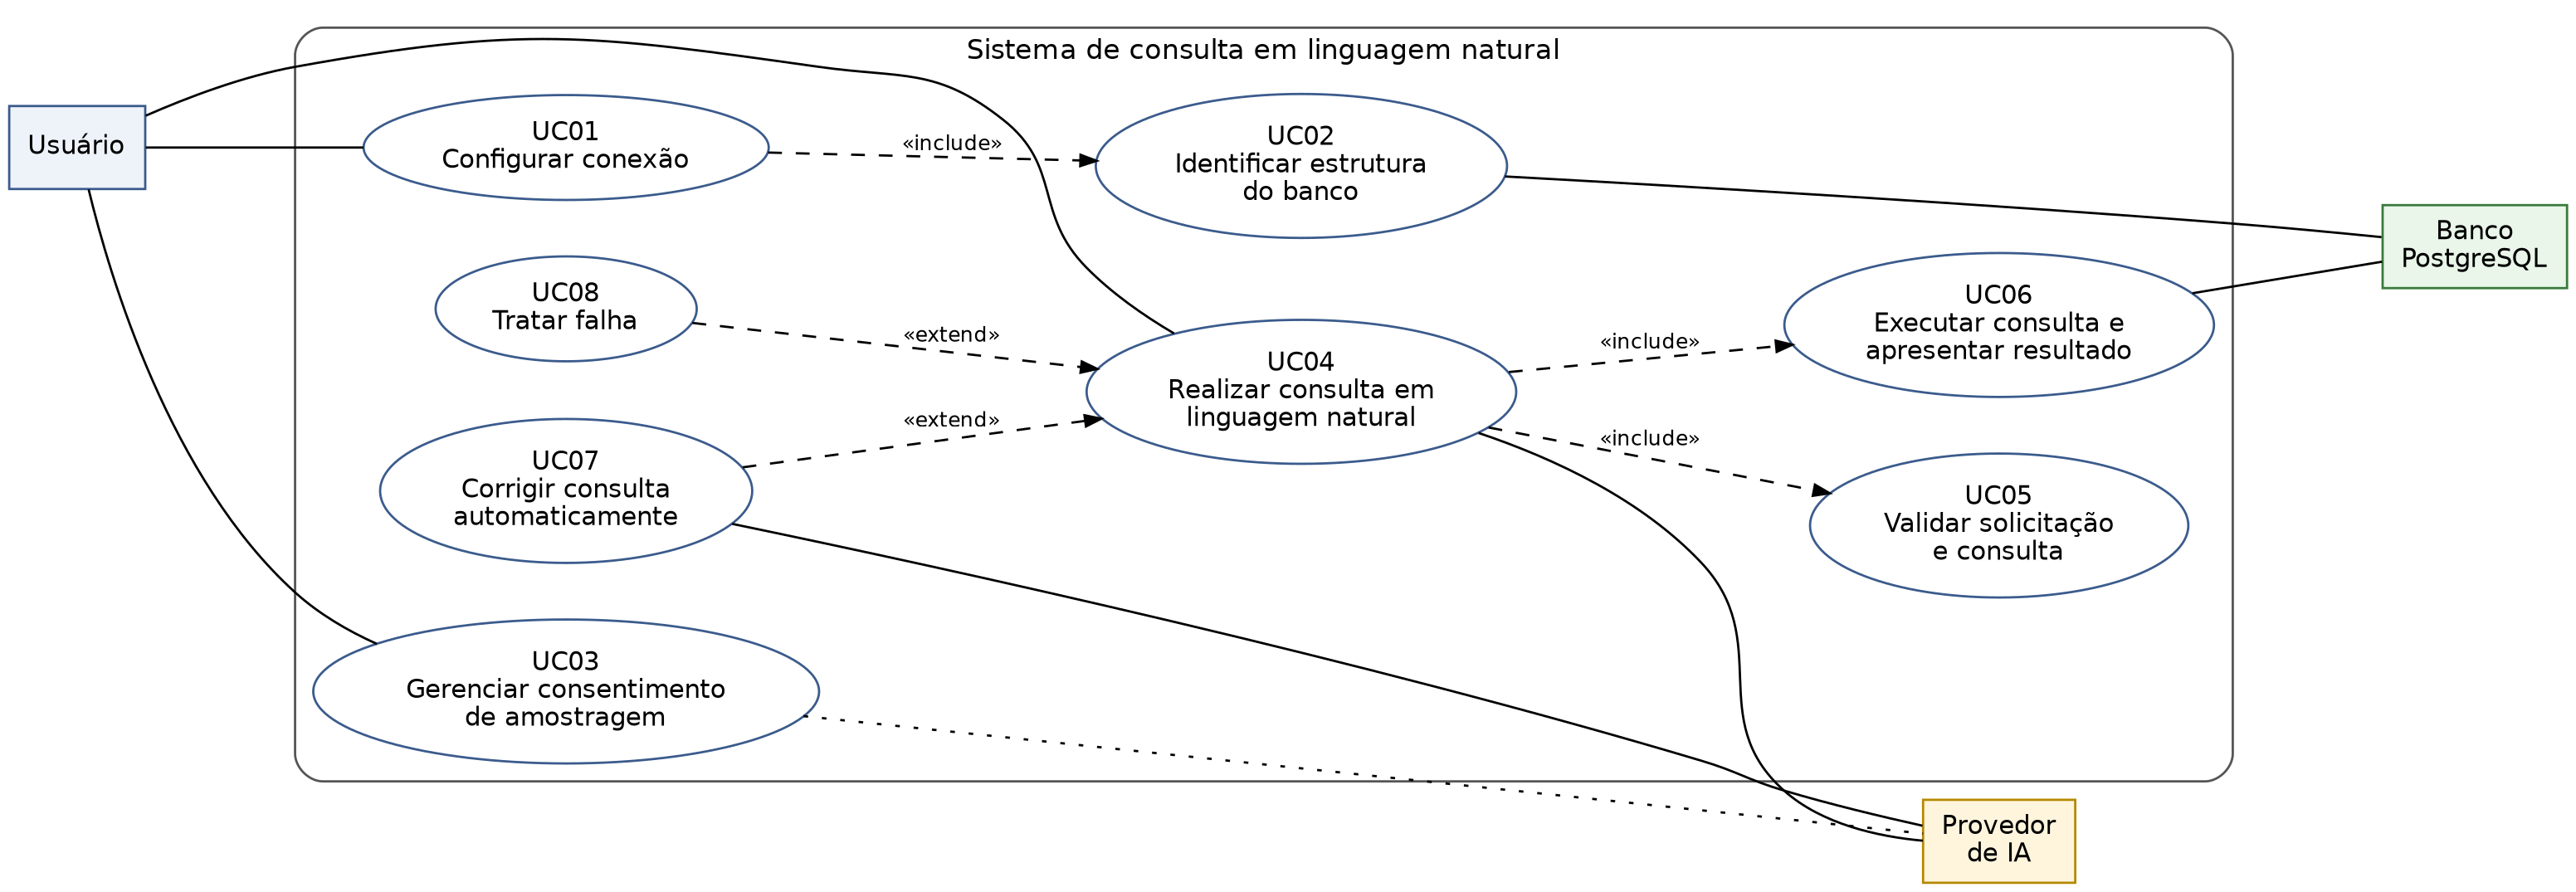
\includegraphics[width=\textwidth]{imagens/casos_de_uso.png}
    \legend{Fonte: Elaborado pelos autores (2026).}
\end{figure}

\begin{quadro}[htb]
    \caption{Casos de uso e requisitos atendidos}
    \label{qua:casos-uso}
    \begin{tabular}{|p{1.5cm}|p{6.2cm}|p{3.0cm}|p{3.5cm}|}
        \hline
        \textbf{Código} & \textbf{Caso de uso} & \textbf{Requisitos} & \textbf{Ator(es)} \\ \hline
        UC01 & Configurar conexão com o banco & RF01 & Usuário \\ \hline
        UC02 & Identificar estrutura do banco & RF02, RF03 & Banco PostgreSQL \\ \hline
        UC03 & Gerenciar consentimento de amostragem & RF04, RF05 & Usuário, Provedor de IA \\ \hline
        UC04 & Realizar consulta em linguagem natural & RF06, RF08 & Usuário, Provedor de IA \\ \hline
        UC05 & Validar solicitação e consulta & RF07, RNF01 & (interno) \\ \hline
        UC06 & Executar consulta e apresentar resultado & RF09, RF10 & Banco PostgreSQL \\ \hline
        UC07 & Corrigir consulta automaticamente & RF11 & Provedor de IA \\ \hline
        UC08 & Tratar falha & RF12, RNF06 & Usuário \\ \hline
    \end{tabular}
    \legend{Fonte: Elaborado pelos autores (2026).}
\end{quadro}

\subsection{UC01 -- Configurar conexão com o banco}

\begin{description}
    \item[Objetivo:] permitir que o usuário informe os dados de acesso a um banco PostgreSQL.
    \item[Ator:] Usuário.
    \item[Pré-condição:] a aplicação está em execução.
    \item[Pós-condição:] conexão estabelecida e estrutura do banco identificada (UC02).
\end{description}

\textbf{Fluxo principal:}
\begin{enumerate}
    \item O usuário informa os dados de conexão (servidor, porta, banco, usuário e senha).
    \item O sistema tenta estabelecer a conexão.
    \item O sistema aciona a identificação da estrutura do banco (UC02).
    \item O sistema informa que o banco está pronto para receber perguntas.
\end{enumerate}

\textbf{Fluxo alternativo:} se a conexão falhar (dados incorretos ou banco inacessível), o sistema informa o erro ao usuário e permite corrigir os dados (RNF06).

\subsection{UC02 -- Identificar estrutura do banco}

\begin{description}
    \item[Objetivo:] levantar automaticamente a estrutura acessível do banco, sem depender do modelo de linguagem.
    \item[Ator:] Banco PostgreSQL.
    \item[Pré-condição:] conexão estabelecida (UC01).
    \item[Pós-condição:] representação estruturada com esquemas, tabelas, colunas, tipos, chaves primárias e estrangeiras disponível para composição do contexto.
\end{description}

\textbf{Fluxo principal:}
\begin{enumerate}
    \item O sistema lista os esquemas acessíveis às credenciais informadas (RF02).
    \item Para cada esquema, o sistema obtém tabelas, colunas, tipos de dados, chaves primárias e chaves estrangeiras (RF03).
    \item O sistema organiza as informações em uma representação estruturada.
\end{enumerate}

\subsection{UC03 -- Gerenciar consentimento de amostragem}

\begin{description}
    \item[Objetivo:] permitir que o usuário autorize ou recuse o envio de amostras de registros ao provedor de IA.
    \item[Ator:] Usuário.
    \item[Pré-condição:] estrutura do banco identificada (UC02).
    \item[Pós-condição:] preferência de amostragem registrada para a sessão.
\end{description}

\textbf{Fluxo principal:}
\begin{enumerate}
    \item O sistema informa que as amostras podem conter dados sensíveis e solicita autorização explícita (RF04).
    \item O usuário autoriza a utilização das amostras.
    \item Quando necessário, o sistema coleta amostras de, no máximo, dez registros por operação (RF05) e as inclui no contexto.
\end{enumerate}

\textbf{Fluxo alternativo:} se o usuário recusar, nenhum registro é lido para composição do contexto e o sistema opera apenas com os metadados estruturais (RNF03).

\subsection{UC04 -- Realizar consulta em linguagem natural}

\begin{description}
    \item[Objetivo:] obter dados do banco a partir de uma pergunta escrita em linguagem natural.
    \item[Atores:] Usuário e Provedor de IA.
    \item[Pré-condição:] banco conectado e estrutura identificada.
    \item[Pós-condição:] resultado apresentado em formato tabular, ou falha informada de forma controlada.
\end{description}

\textbf{Fluxo principal:}
\begin{enumerate}
    \item O usuário digita uma pergunta em linguagem natural (RF06).
    \item O sistema prepara o contexto com a estrutura do banco e, se autorizadas, as amostras.
    \item O sistema verifica se a solicitação é compatível com o escopo de leitura (UC05).
    \item O sistema solicita ao provedor de IA a geração da consulta SQL (RF08).
    \item O sistema valida a consulta gerada (UC05).
    \item O sistema executa a consulta aprovada e apresenta o resultado em tabela (UC06).
\end{enumerate}

\textbf{Fluxos alternativos:}
\begin{enumerate}
    \item[A1.] \emph{Solicitação incompatível:} se a pergunta exigir inserção, atualização, exclusão ou alteração estrutural, o sistema não prossegue para a execução e informa o motivo ao usuário (RF07).
    \item[A2.] \emph{Consulta reprovada na validação:} a consulta não é executada; o sistema pode solicitar nova geração dentro do limite de tentativas (UC07) ou, esgotado o limite, tratar a falha (UC08).
    \item[A3.] \emph{Erro de geração ou execução:} o sistema aciona a correção automática (UC07).
\end{enumerate}

\subsection{UC05 -- Validar solicitação e consulta}

Caso de uso incluído em UC04. O sistema verifica a intenção da pergunta (RF07) e, após a geração, analisa a consulta produzida por uma camada de validação independente do modelo, aprovando apenas uma instrução \texttt{SELECT} e bloqueando comandos de escrita ou de alteração estrutural (RN01 a RN03; RNF01).

\subsection{UC06 -- Executar consulta e apresentar resultado}

Caso de uso incluído em UC04. O sistema executa a consulta aprovada em modo somente leitura (RF09; RN04), processa o resultado e o apresenta ao usuário em formato tabular na interface gráfica (RF10), registrando latência e demais informações de execução (RNF07).

\subsection{UC07 -- Corrigir consulta automaticamente}

Caso de uso que estende UC04. Quando uma consulta permitida falha na geração ou na execução, o sistema envia o erro ao provedor de IA e obtém uma nova versão da consulta, repetindo o processo em até três tentativas (RF11; RN08). Cada tentativa é registrada para fins de avaliação (RN10).

\subsection{UC08 -- Tratar falha}

Caso de uso que estende UC04. Esgotado o limite de tentativas, ou diante de falhas de conexão ou de comunicação com o provedor de IA, o sistema encerra a operação de maneira controlada e informa a falha ao usuário, sem executar consultas não aprovadas (RF12; RNF06).

\section{Rastreabilidade dos Requisitos}
\label{ap:rastreabilidade}

O Quadro~\ref{qua:rastreabilidade} relaciona os requisitos funcionais aos casos de uso e aos incrementos em que são implementados. O fluxo essencial é validado tecnicamente na V0 e integrado à interface gráfica na V1.

\begin{quadro}[htb]
    \caption{Rastreabilidade dos requisitos funcionais}
    \label{qua:rastreabilidade}
    \begin{tabular}{|p{1.4cm}|p{7.2cm}|p{2.2cm}|p{2.8cm}|}
        \hline
        \textbf{Req.} & \textbf{Descrição resumida} & \textbf{Caso de uso} & \textbf{Incremento} \\ \hline
        RF01 & Conexão com banco de dados & UC01 & V0 e V1 \\ \hline
        RF02 & Identificação de esquemas & UC02 & V0 e V1 \\ \hline
        RF03 & Introspecção estrutural & UC02 & V0 e V1 \\ \hline
        RF04 & Consentimento para amostragem & UC03 & V1 \\ \hline
        RF05 & Limitação das amostras & UC03 & V1 \\ \hline
        RF06 & Entrada em linguagem natural & UC04 & V0 e V1 \\ \hline
        RF07 & Validação da intenção & UC04, UC05 & V0 e V1 \\ \hline
        RF08 & Geração de consulta SQL & UC04 & V0 e V1 \\ \hline
        RF09 & Execução da consulta & UC06 & V0 e V1 \\ \hline
        RF10 & Apresentação do resultado & UC06 & V0 e V1 \\ \hline
        RF11 & Correção automática de consultas & UC07 & V1 \\ \hline
        RF12 & Tratamento de falha & UC08 & V1 \\ \hline
    \end{tabular}
    \legend{Fonte: Elaborado pelos autores (2026).}
\end{quadro}

\section{Critérios de Verificação dos Requisitos Não Funcionais}
\label{ap:criterios-rnf}

O Quadro~\ref{qua:criterios-rnf} indica como cada requisito não funcional será verificado durante a validação do sistema.

\begin{quadro}[htb]
    \caption{Critérios de verificação dos requisitos não funcionais}
    \label{qua:criterios-rnf}
    \begin{tabular}{|p{1.7cm}|p{4.0cm}|p{8.5cm}|}
        \hline
        \textbf{Req.} & \textbf{Requisito} & \textbf{Forma de verificação} \\ \hline
        RNF01 & Segurança & Conjunto de solicitações e consultas proibidas; medição da taxa de bloqueio correto. \\ \hline
        RNF02 & Privacidade & Inspeção do contexto enviado ao provedor, verificando a ausência de registros sem consentimento. \\ \hline
        RNF03 & Independência da amostragem & Execução do fluxo principal com a amostragem recusada. \\ \hline
        RNF04 & Modularidade & Revisão da arquitetura quanto à separação entre introspecção, contexto, geração, validação, execução e apresentação. \\ \hline
        RNF05 & Baixo acoplamento ao modelo & Substituição do provedor de IA sem alteração dos demais módulos. \\ \hline
        RNF06 & Tratamento de erros & Simulação de falhas de conexão, de provedor, de geração e de execução. \\ \hline
        RNF07 & Observabilidade & Verificação dos registros de latência, erros, tentativas e execuções. \\ \hline
        RNF08 & Usabilidade & Execução do fluxo principal pela interface desktop, sem uso de terminal ou código-fonte. \\ \hline
    \end{tabular}
    \legend{Fonte: Elaborado pelos autores (2026).}
\end{quadro}
	
	
	
	% ----------------------------------------------------------
	\chapter{Modelo Estrutural do Sistema}
	% ----------------------------------------------------------

  \label{ap:estrutural}

Este apêndice apresenta o modelo estrutural do sistema por meio de diagramas de classes da UML. Optou-se por dois diagramas complementares: o modelo de domínio, que representa as informações manipuladas pela aplicação, e o modelo de módulos do backend, que representa as classes responsáveis por cada etapa do fluxo descrito na Seção~\ref{sec:visao-geral}. Os nomes seguem a nomenclatura de implementação prevista e podem ser refinados durante o desenvolvimento.

\section{Modelo de Domínio}
\label{ap:dominio}

A Figura~\ref{fig:dominio} apresenta as principais classes de domínio. A estrutura do banco é obtida a partir de uma conexão e composta por esquemas, tabelas, colunas e chaves estrangeiras, obtidos de forma determinística pelo módulo de introspecção. As amostras de registros são opcionais e associadas às tabelas somente quando o usuário as autoriza. O contexto de consulta reúne a estrutura, as amostras eventuais e a pergunta, e serve de base para a geração da consulta SQL, que passa por validação e, quando aprovada, produz um resultado.

\begin{figure}[htb]
    \centering
    \caption{Diagrama de classes -- modelo de domínio}
    \label{fig:dominio}
    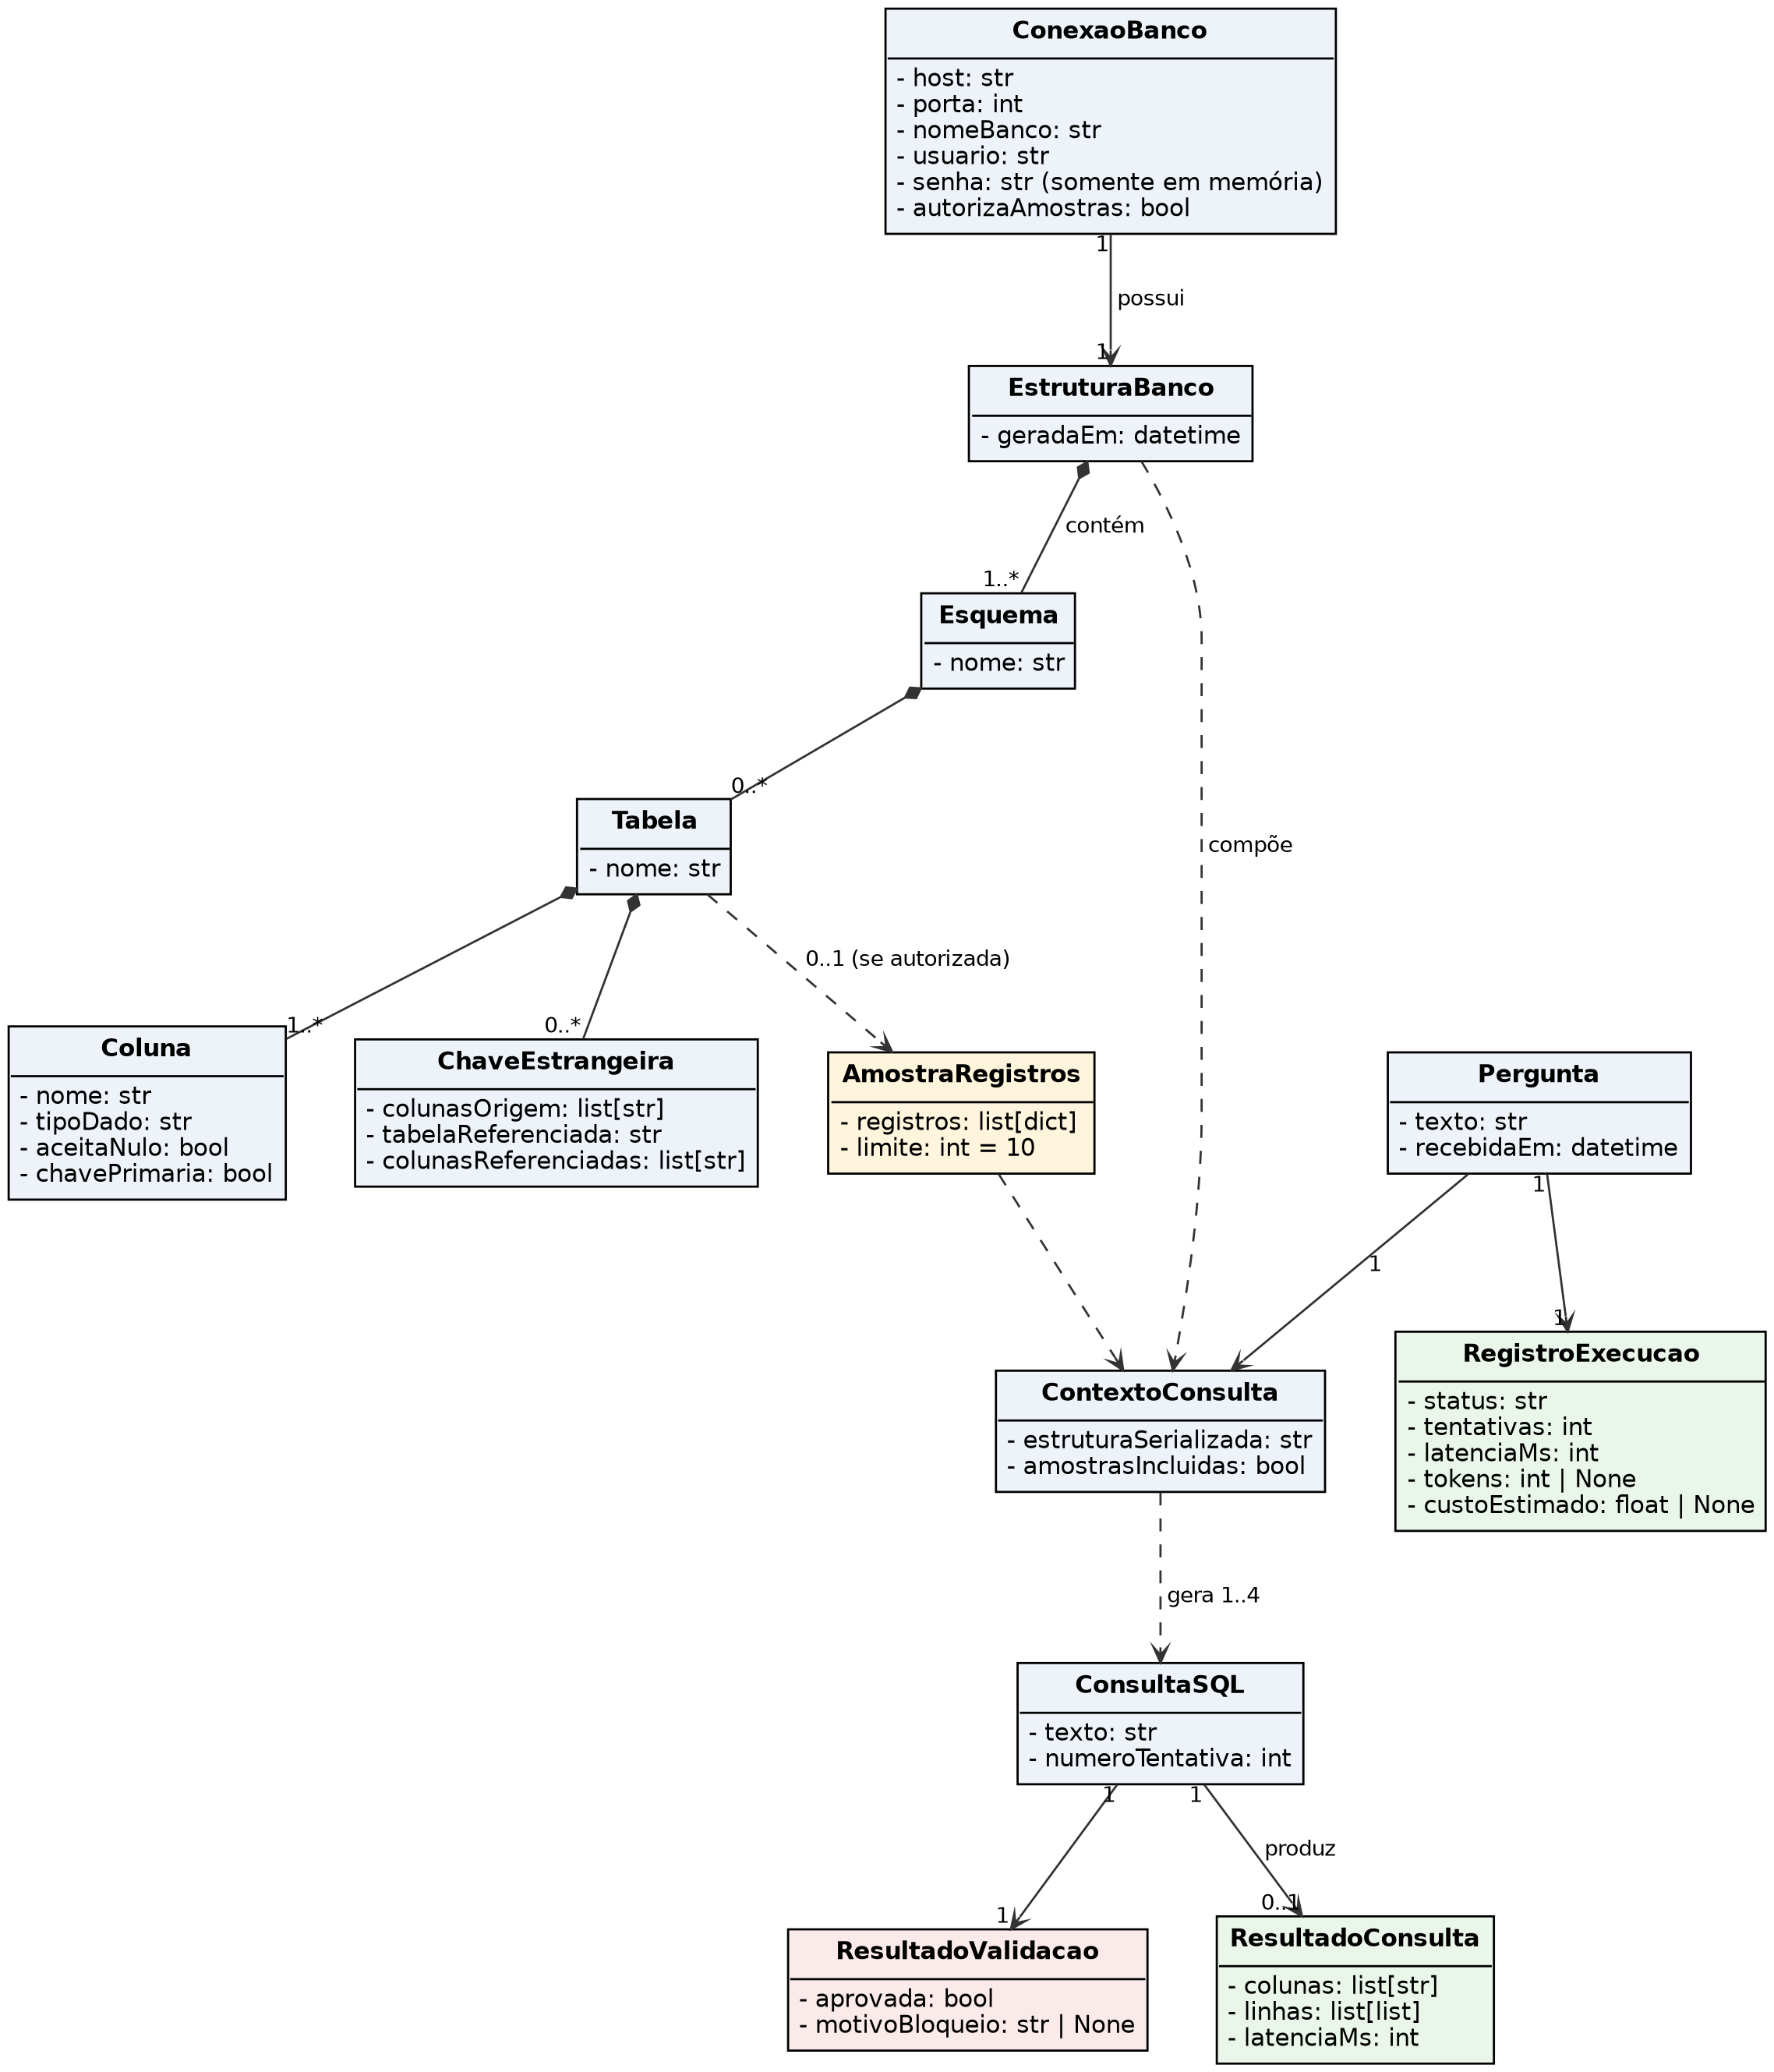
\includegraphics[width=\textwidth]{imagens/diagrama_classes_dominio.png}
    \legend{Fonte: Elaborado pelos autores (2026).}
\end{figure}

O Quadro~\ref{qua:classes-dominio} descreve a responsabilidade de cada classe.

\begin{quadro}[htb]
    \caption{Classes do modelo de domínio}
    \label{qua:classes-dominio}
    \begin{tabular}{|p{3.6cm}|p{10.6cm}|}
        \hline
        \textbf{Classe} & \textbf{Responsabilidade} \\ \hline
        ConexaoBanco & Dados de acesso ao PostgreSQL informados pelo usuário e sua decisão sobre o uso de amostras (RF01, RF04). A senha é mantida apenas em memória durante a sessão. \\ \hline
        EstruturaBanco & Representação estruturada de tudo o que foi identificado na introspecção (RF02, RF03). \\ \hline
        Esquema, Tabela, Coluna & Elementos estruturais do banco, incluindo tipo de dado, aceitação de nulos e indicação de chave primária. \\ \hline
        ChaveEstrangeira & Relacionamento entre tabelas, usado para que a geração de SQL reconheça junções possíveis. \\ \hline
        AmostraRegistros & Conjunto opcional de registros, limitado a dez por amostragem (RF05), incluído no contexto somente com consentimento. \\ \hline
        Pergunta & Solicitação em linguagem natural formulada pelo usuário (RF06). \\ \hline
        ContextoConsulta & Contexto enviado ao provedor de IA, composto pela estrutura, pelas amostras (se houver) e pela pergunta. \\ \hline
        ConsultaSQL & Consulta gerada pelo modelo, com indicação do número da tentativa, de modo a controlar as correções (RF11). \\ \hline
        ResultadoValidacao & Resultado da análise de segurança: consulta aprovada ou bloqueada, com o motivo (RF07, RNF01). \\ \hline
        ResultadoConsulta & Colunas, linhas e latência da consulta executada (RF09, RF10). \\ \hline
        RegistroExecucao & Informações de observabilidade de cada solicitação: estado final, tentativas, latência e, quando disponíveis, tokens e custo estimado (RNF07). \\ \hline
    \end{tabular}
    \legend{Fonte: Elaborado pelos autores (2026).}
\end{quadro}

\section{Modelo de Módulos do Backend}
\label{ap:modulos}

A Figura~\ref{fig:servicos} apresenta as classes de serviço do backend em Python e FastAPI. Cada uma concentra uma etapa do fluxo, atendendo ao requisito de modularidade (RNF04). O \texttt{OrquestradorConsulta} coordena a sequência de etapas e é o único componente que conhece a ordem do fluxo. A comunicação com o provedor de inteligência artificial ocorre exclusivamente por meio da interface \texttt{ProvedorLLM}, implementada por classes específicas de cada provedor, o que permite a substituição do modelo sem alterar as demais classes (RNF05).

\begin{figure}[htb]
    \centering
    \caption{Diagrama de classes -- módulos do backend}
    \label{fig:servicos}
    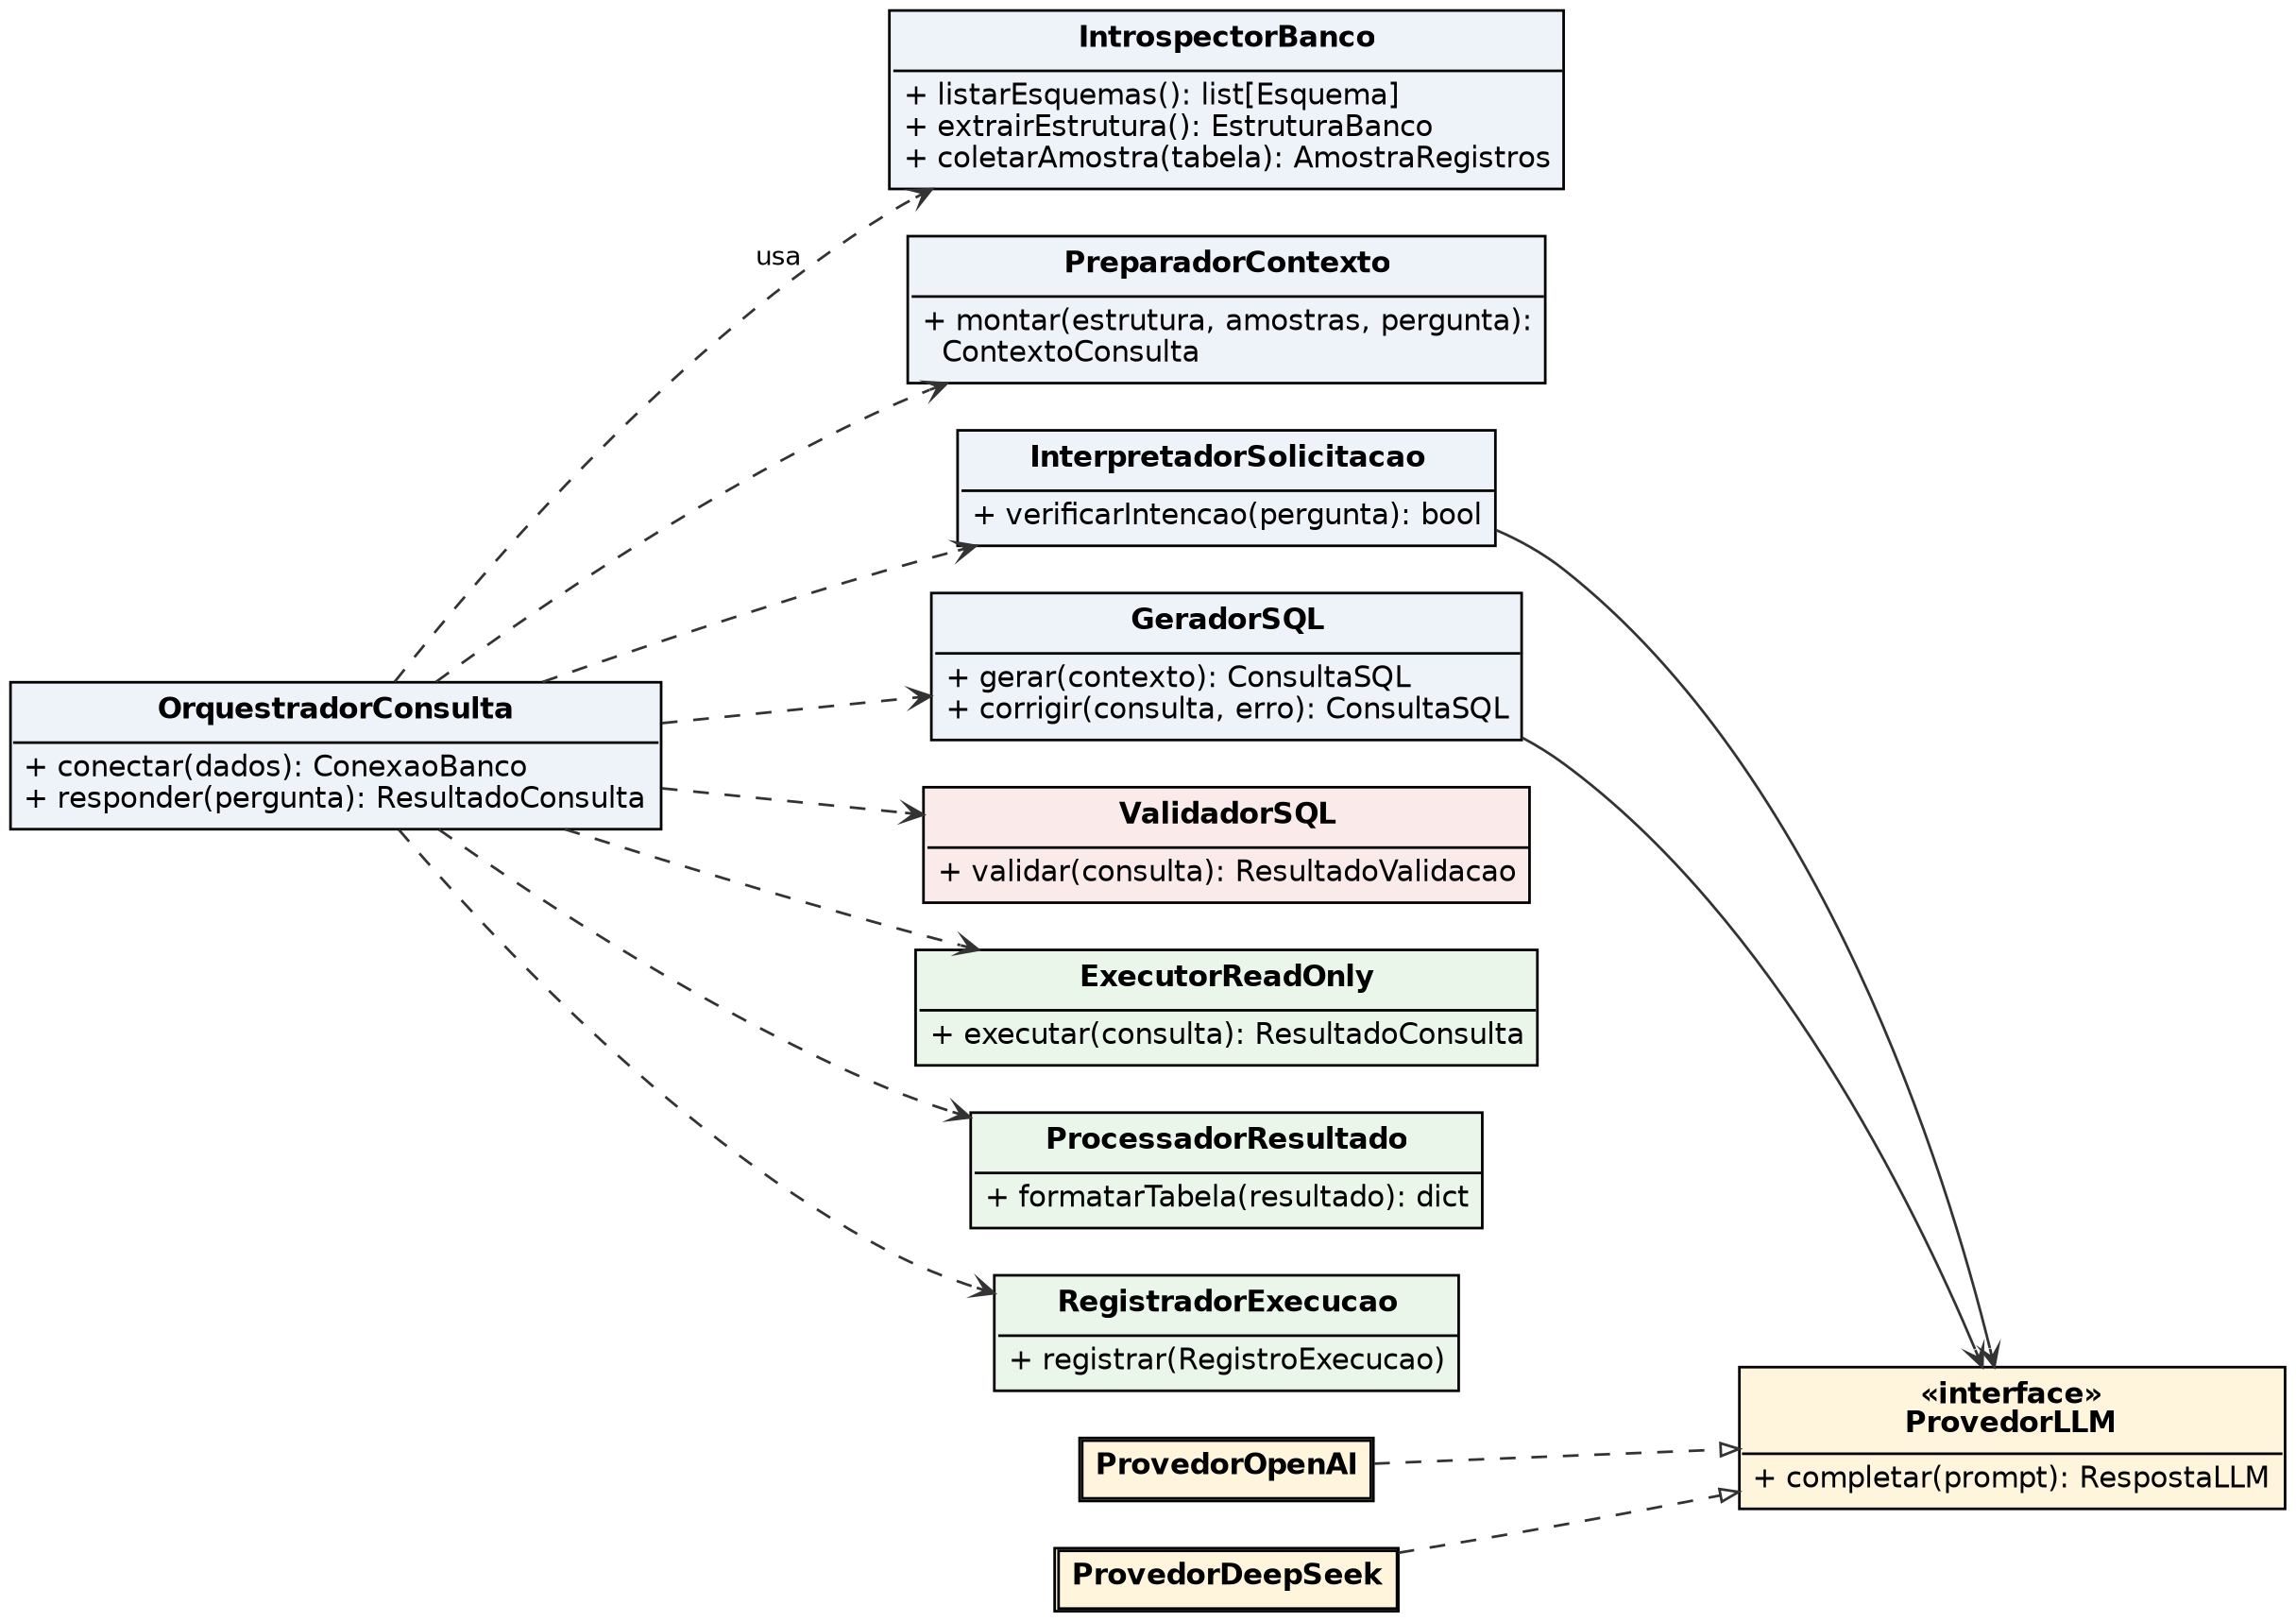
\includegraphics[width=\textwidth]{imagens/diagrama_classes_servicos.png}
    \legend{Fonte: Elaborado pelos autores (2026).}
\end{figure}

\begin{quadro}[htb]
    \caption{Classes de serviço do backend}
    \label{qua:classes-servicos}
    \begin{tabular}{|p{4.0cm}|p{10.2cm}|}
        \hline
        \textbf{Classe} & \textbf{Responsabilidade} \\ \hline
        OrquestradorConsulta & Coordena o fluxo completo, do recebimento da pergunta à entrega do resultado, incluindo o controle do limite de tentativas de correção. \\ \hline
        IntrospectorBanco & Módulo de descoberta (\textit{crawler}): lista esquemas, extrai a estrutura e, quando autorizado, coleta as amostras. \\ \hline
        PreparadorContexto & Monta o contexto enviado ao modelo a partir da estrutura, das amostras e da pergunta. \\ \hline
        InterpretadorSolicitacao & Identifica solicitações incompatíveis com o escopo de leitura (RF07). \\ \hline
        GeradorSQL & Gera a consulta SQL e, em caso de erro, solicita sua correção (RF08, RF11). \\ \hline
        ProvedorLLM (interface) & Contrato de comunicação com o modelo de linguagem, implementado por ProvedorOpenAI e ProvedorDeepSeek. \\ \hline
        ValidadorSQL & Camada de guardrails independente do modelo: aprova apenas consultas de leitura e bloqueia as demais (RNF01). \\ \hline
        ExecutorReadOnly & Executa a consulta aprovada em modo somente leitura (RF09). \\ \hline
        ProcessadorResultado & Converte o resultado para o formato entregue à interface (RF10). \\ \hline
        RegistradorExecucao & Registra latência, erros, tentativas e execuções (RNF07). \\ \hline
    \end{tabular}
    \legend{Fonte: Elaborado pelos autores (2026).}
\end{quadro}

\section{Considerações sobre o Modelo}
\label{ap:consideracoes-modelo}

As classes de domínio serão implementadas como modelos Pydantic, que definem contratos explícitos de entrada e saída da API e validam os dados trocados entre a interface e o backend. O acesso ao PostgreSQL e a introspecção utilizarão o SQLAlchemy. Diagramas complementares de comportamento, arquitetura e dados são apresentados nos apêndices seguintes.

	
	
	
	% ----------------------------------------------------------
	\chapter{Modelo Comportamental do Sistema}
	% ----------------------------------------------------------
   
    Texto de apresentação do Apêndice - Fluxograma ou Diagrama de Sequência ou Diagrama de Estados..
	
	
	
	% ----------------------------------------------------------
	\chapter{Modelo da Arquitetura do Sistema}
	% ----------------------------------------------------------
	
	Texto de apresentação do Apêndice - Diagrama de blocos de alto nível ou Diagrama de Componentes.
	
	
	% ----------------------------------------------------------
	\chapter{Modelo de Dados do Sistema}
	% ----------------------------------------------------------
	
    Texto de apresentação do Apêndice - Modelo Entidade-Relacionamento e Diagrama Entidade-Relacionamento.

    % ----------------------------------------------------------
	\chapter{Outro Apêndice}
	% ----------------------------------------------------------
	
	Texto do Apêndice adicional.



 
\end{apendicesenv}